\chapter[Measuring FD PMT Gain Variance with CalA Data]{\centering Measuring FD PMT Gain Variance with CalA Data \\}\label{Ch:GainVariance}

Measuring Gain Variance of FD PMT with CalA Data
\begin{itemize}
\item Measuring Gain Variance in the lab did not work. Equipment was not sensitive enough to the low current.
\item There was issues with calibrating the LED light source with another PMT (QE curve and wavelength response not the same?)
\item Using Low/Standard measurements of CalA to find Gain Variance Ratio
\item Two different methods
\item Bootstrap method to find uncertainties on Method 2
\end{itemize}


\begin{figure} % Electronic Noise Distribution
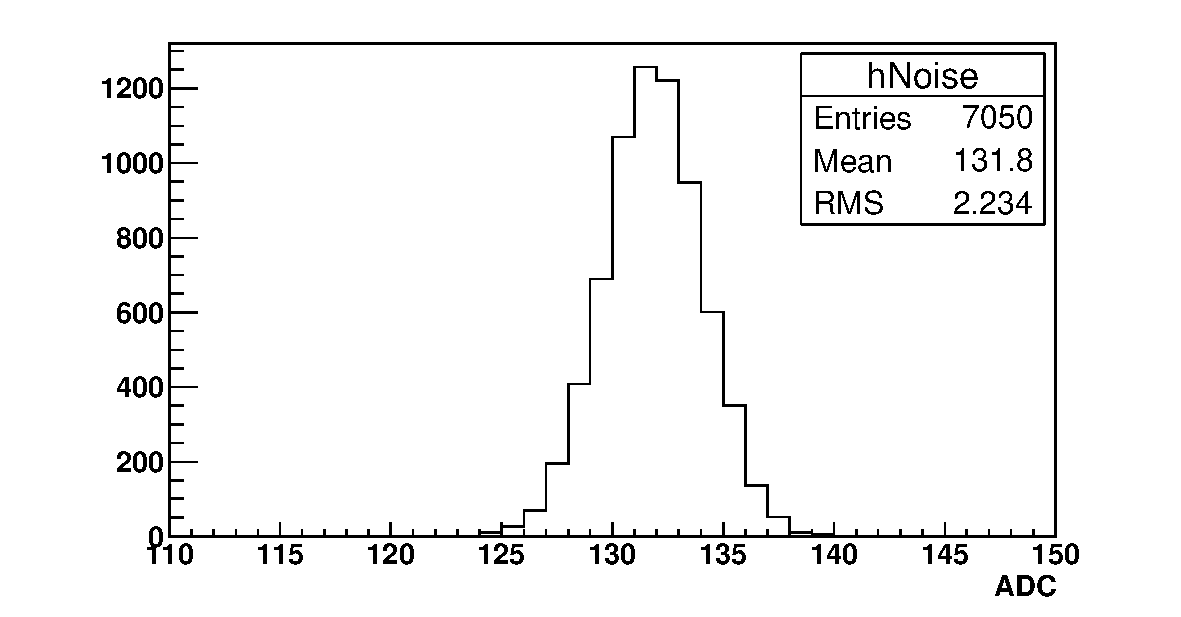
\includegraphics[width=\textwidth]{chapters/graphs/GainVarsMeas/LL_m04_2016-06-11/example_NoiseHist1.pdf}
\caption{}
\vspace{3mm}
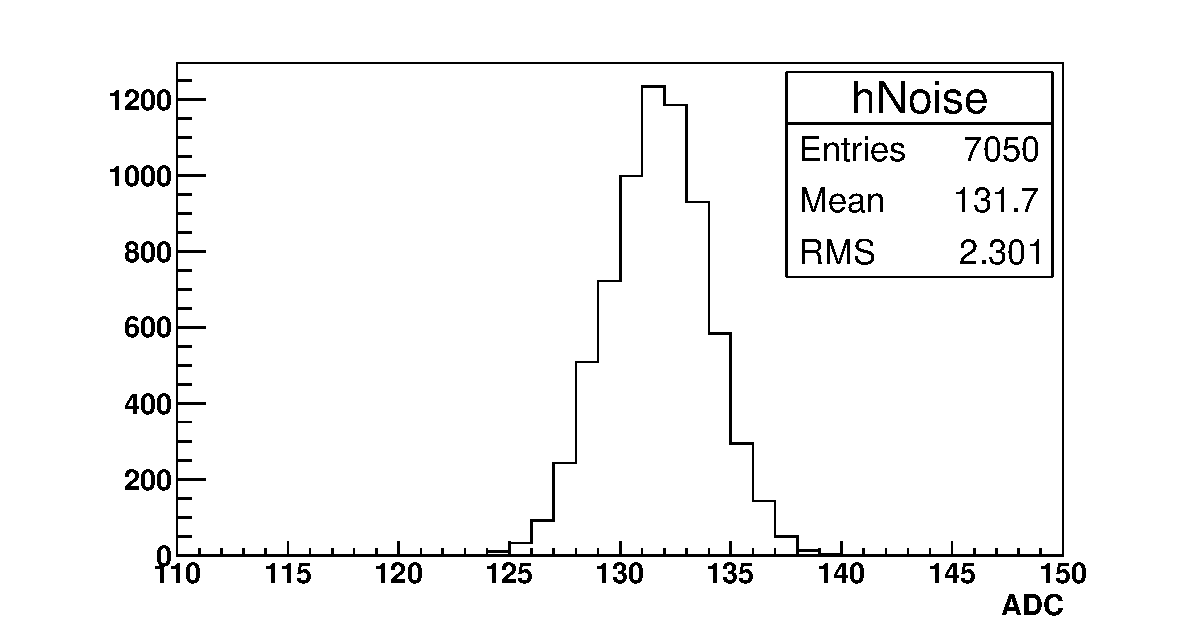
\includegraphics[width=\textwidth]{chapters/graphs/GainVarsMeas/LL_m04_2016-06-11/example_NoiseHist2.pdf}
\caption{}
\end{figure}

\section{Result of Pairs Method}

\begin{figure} % Mean Plot
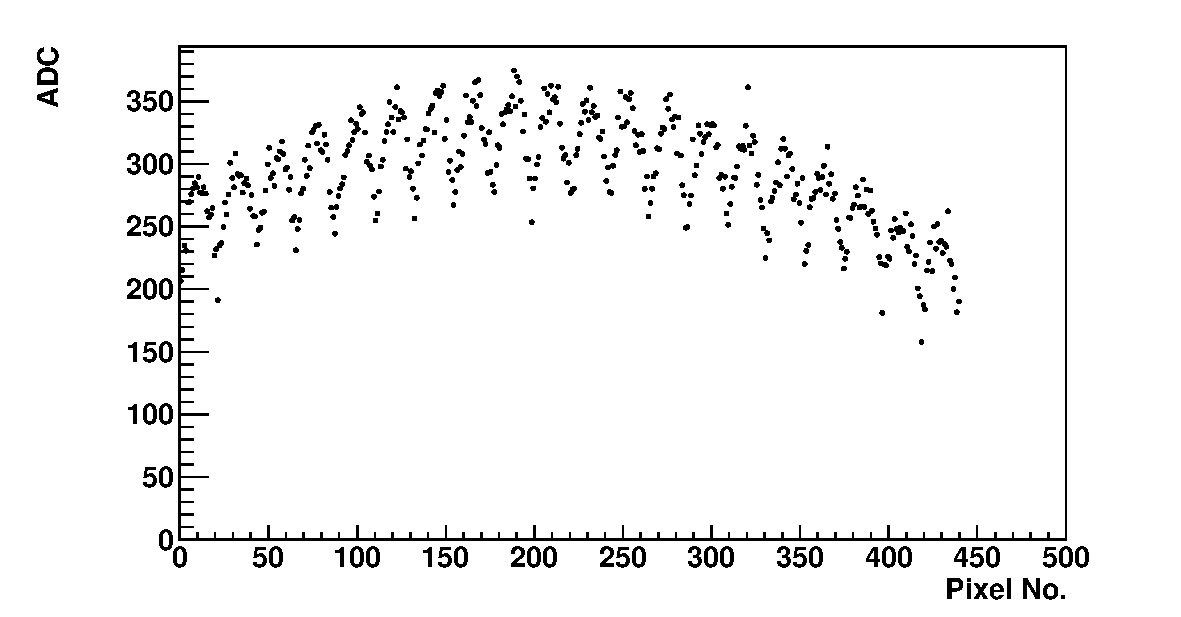
\includegraphics[width=\textwidth]{chapters/graphs/GainVarsMeas/LL_m04_2016-06-11/Set0and2/meanHist_StandHV_Pairs_set0and2.pdf}
\caption{}
\vspace{3mm}
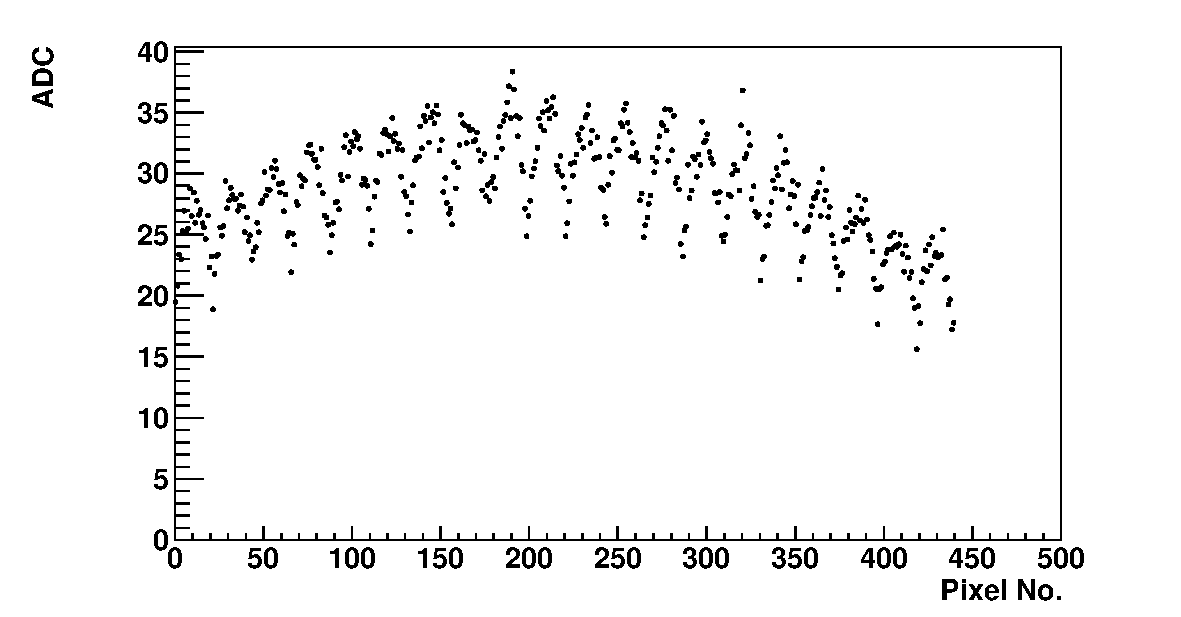
\includegraphics[width=\textwidth]{chapters/graphs/GainVarsMeas/LL_m04_2016-06-11/Set0and2/meanHist_LowHV_Pairs_set0and2.pdf}
\caption{}
\end{figure}

\begin{figure} % Variance Plot
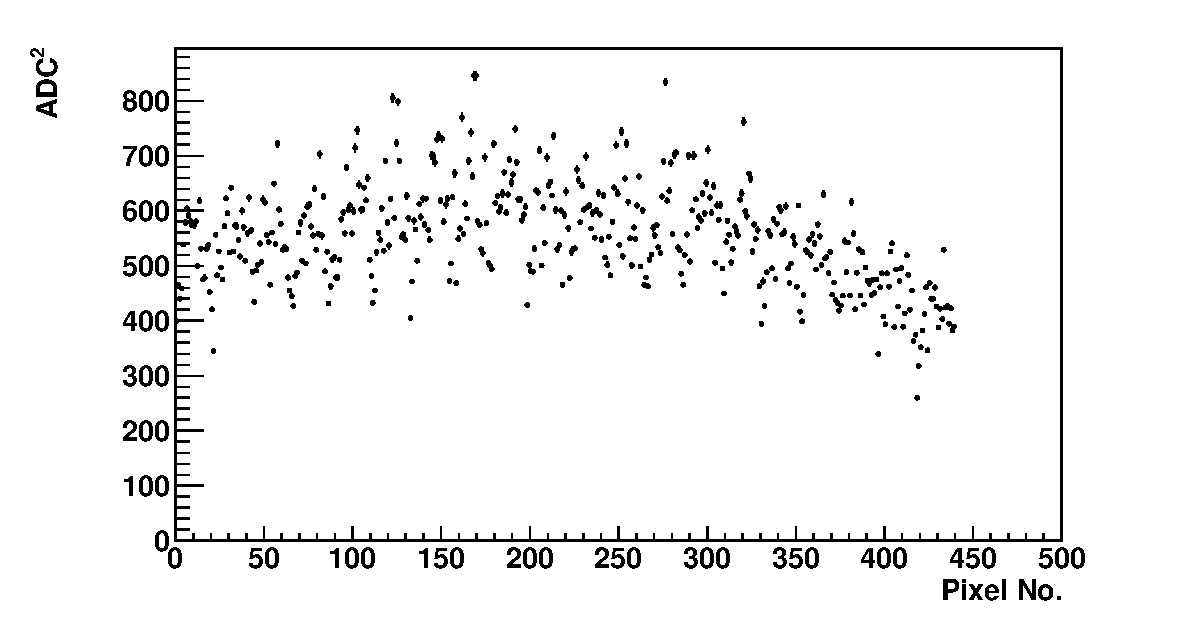
\includegraphics[width=\textwidth]{chapters/graphs/GainVarsMeas/LL_m04_2016-06-11/Set0and2/varianceHist_StandHV_Pairs_set0and2.pdf}
\caption{}
\vspace{3mm}
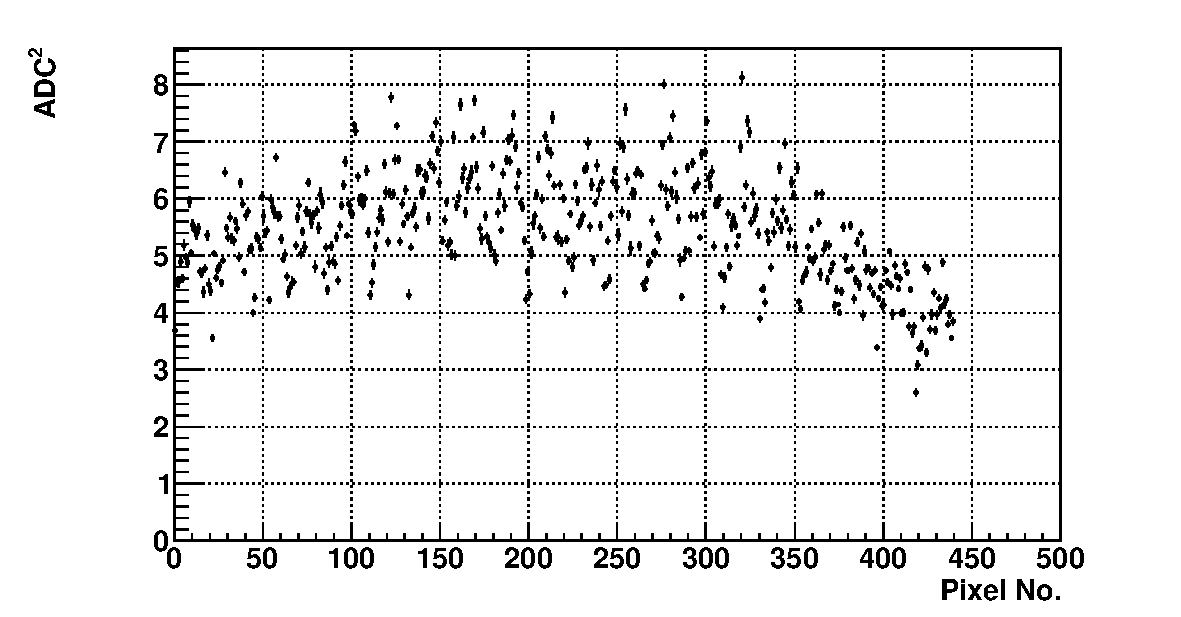
\includegraphics[width=\textwidth]{chapters/graphs/GainVarsMeas/LL_m04_2016-06-11/Set0and2/varianceHist_LowHV_Pairs_set0and2.pdf}
\caption{}
\end{figure}

\begin{figure} % Gain Variance Plot
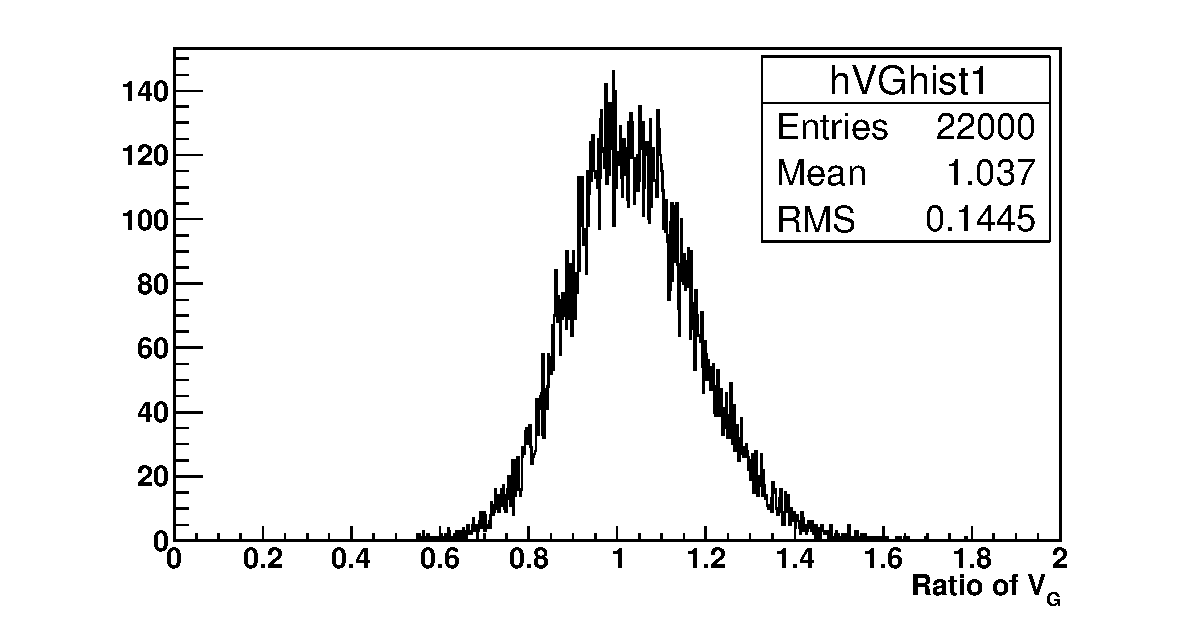
\includegraphics[width=\textwidth]{chapters/graphs/GainVarsMeas/LL_m04_2016-06-11/Set0and2/GainVairanceHist_Pairs.pdf}
\caption{}
\vspace{3mm}
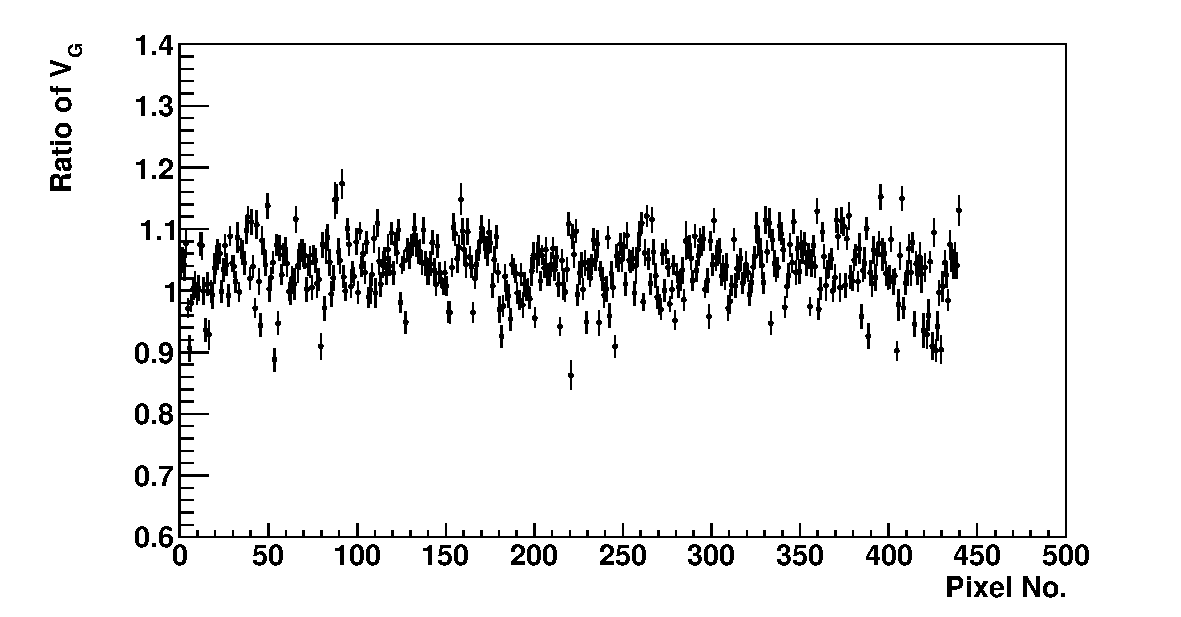
\includegraphics[width=\textwidth]{chapters/graphs/GainVarsMeas/LL_m04_2016-06-11/Set0and2/GainVars_Vs_Pixel_GainVariance_Pairs_Set0and2.pdf}
\caption{}
\end{figure}

\section{Result of Averaging Sets of Traces Method}

\begin{figure} % Mean Plot
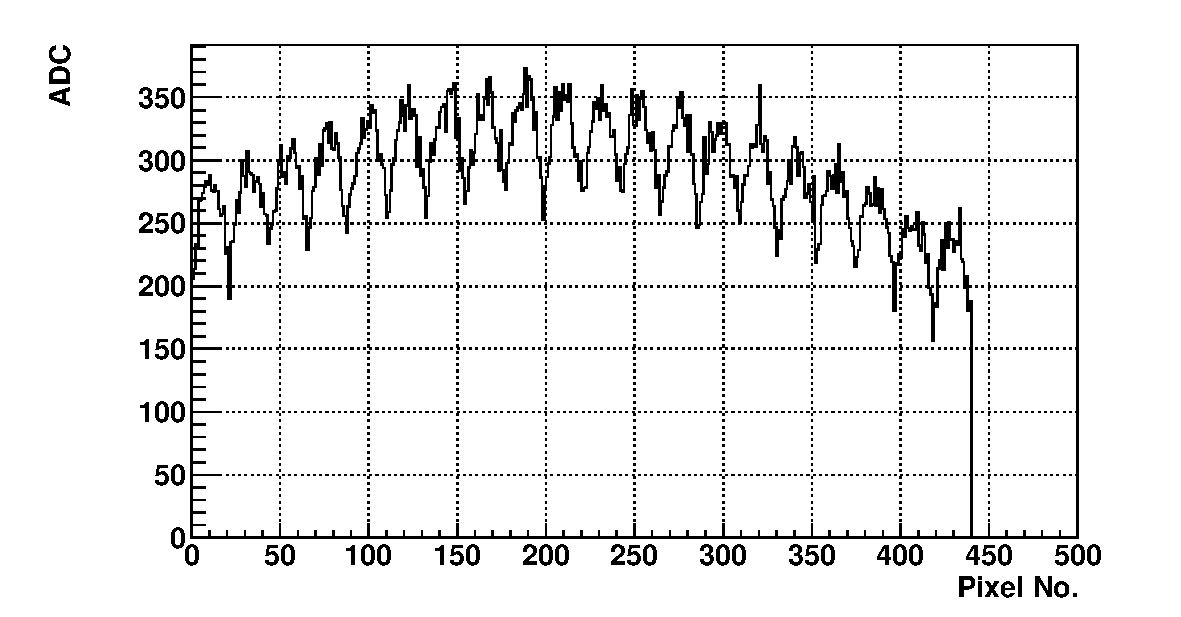
\includegraphics[width=\textwidth]{chapters/graphs/GainVarsMeas/LL_m04_2016-06-11/Set0and2/meanHist_StandHV_Average_set0and2.pdf}
\caption{}
\vspace{3mm}
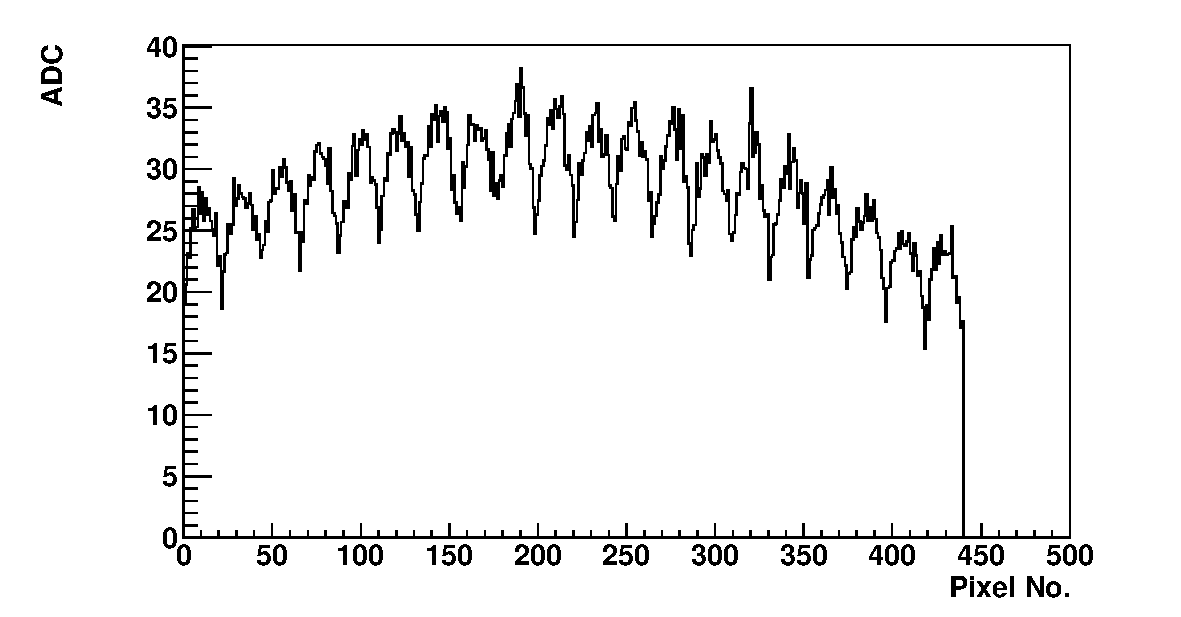
\includegraphics[width=\textwidth]{chapters/graphs/GainVarsMeas/LL_m04_2016-06-11/Set0and2/meanHist_LowHV_Average_set0and2.pdf}
\caption{}
\end{figure}

\begin{figure} % Variance Plot
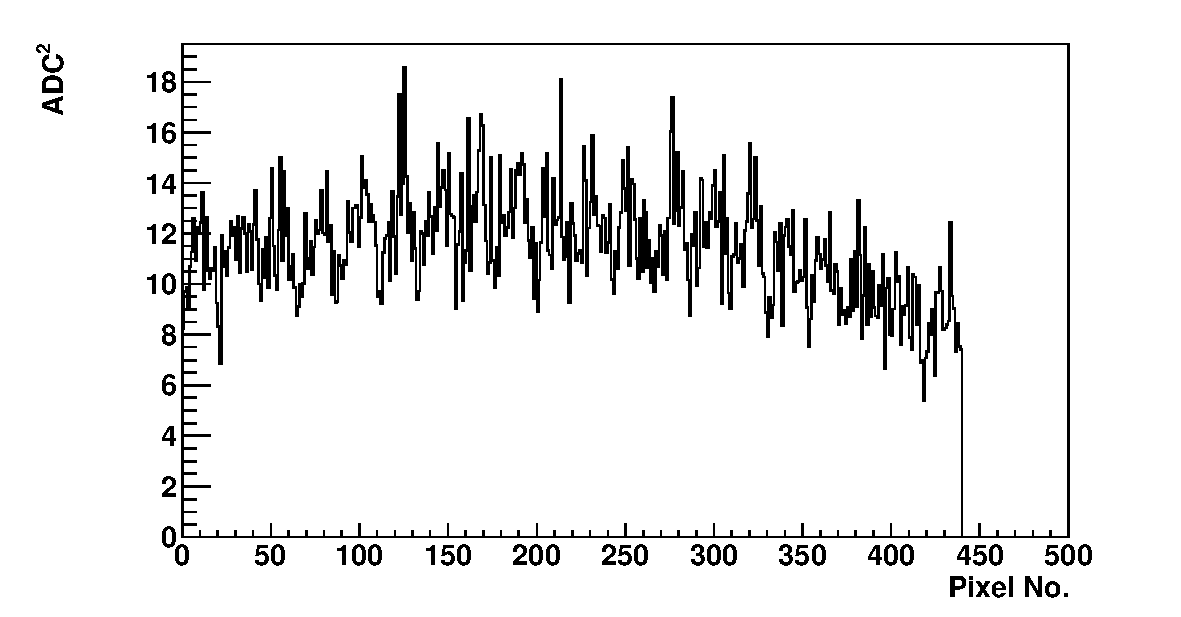
\includegraphics[width=\textwidth]{chapters/graphs/GainVarsMeas/LL_m04_2016-06-11/Set0and2/varianceHist_StandHV_Average_set0and2.pdf}
\caption{}
\vspace{3mm}
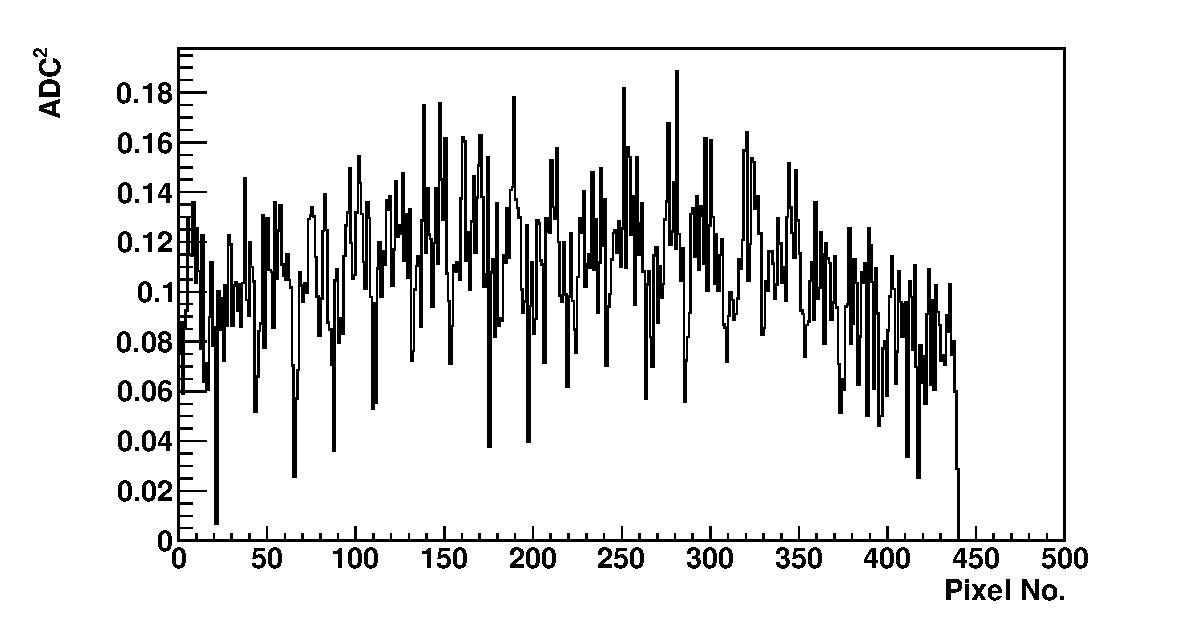
\includegraphics[width=\textwidth]{chapters/graphs/GainVarsMeas/LL_m04_2016-06-11/Set0and2/varianceHist_LowHV_Average_set0and2.pdf}
\caption{}
\end{figure}

\begin{figure} % Gain Variance Plot
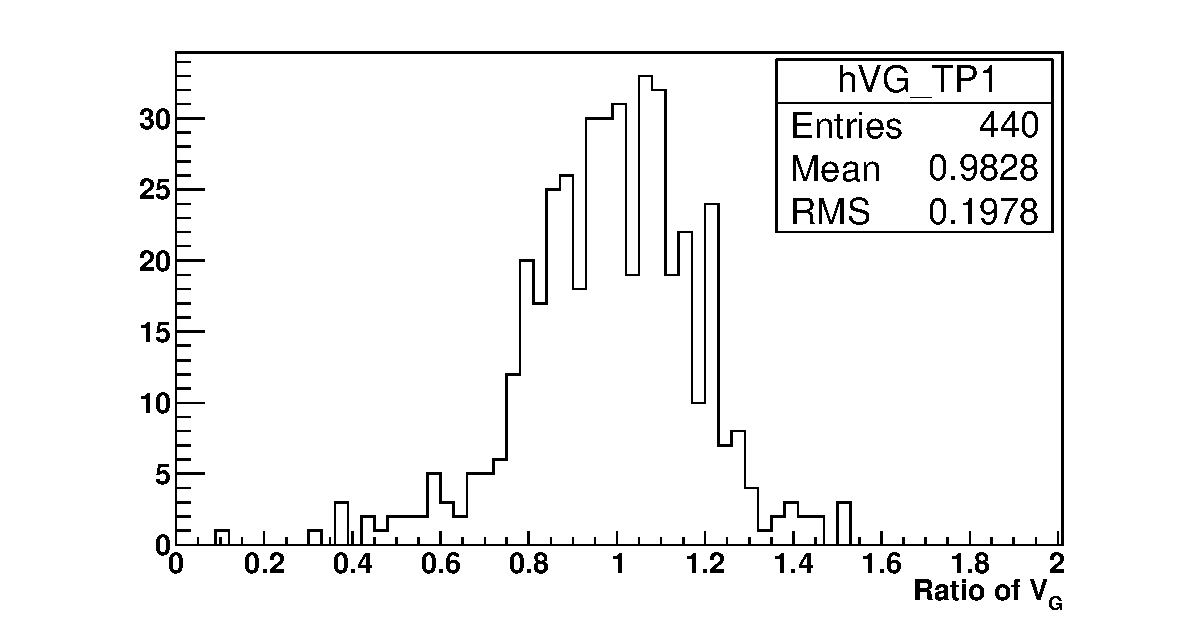
\includegraphics[width=\textwidth]{chapters/graphs/GainVarsMeas/LL_m04_2016-06-11/Set0and2/GainVairanceHist_Average_Method1.pdf}
\caption{}
\vspace{3mm}
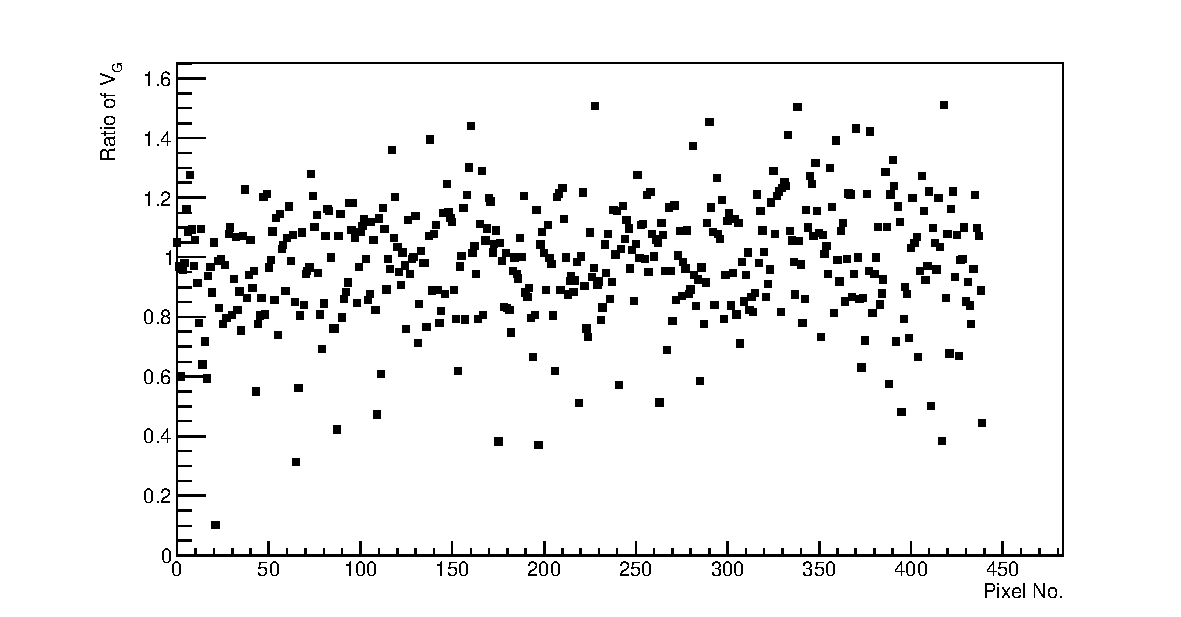
\includegraphics[width=\textwidth]{chapters/graphs/GainVarsMeas/LL_m04_2016-06-11/Set0and2/GainVars_Vs_Pixel_GainVariance_Average_Method1_Set0and2.pdf}
\caption{}
\end{figure}

\section{Result of Averaging Sets of Traces Method with Least Trimmed Squares}

\begin{figure}% Signal Chi2
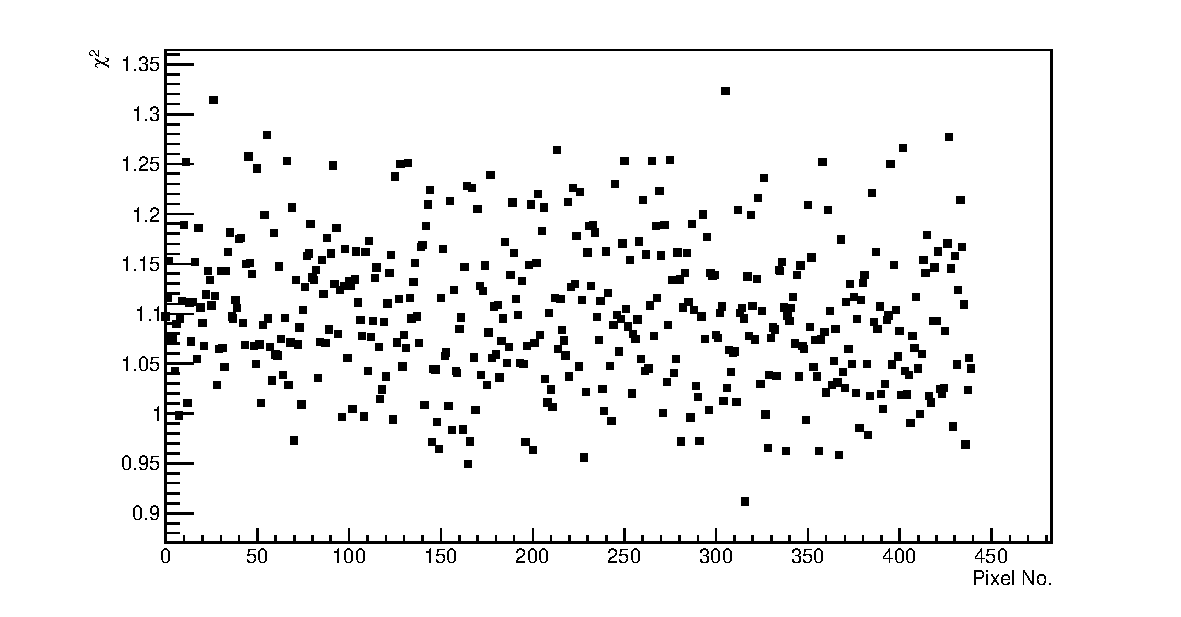
\includegraphics[width=\textwidth]{chapters/graphs/GainVarsMeas/LL_m04_2016-06-11/Set0and2/Chi2_AverageMethod_Signal_StandHV.pdf}
\caption{}
\vspace{3mm}
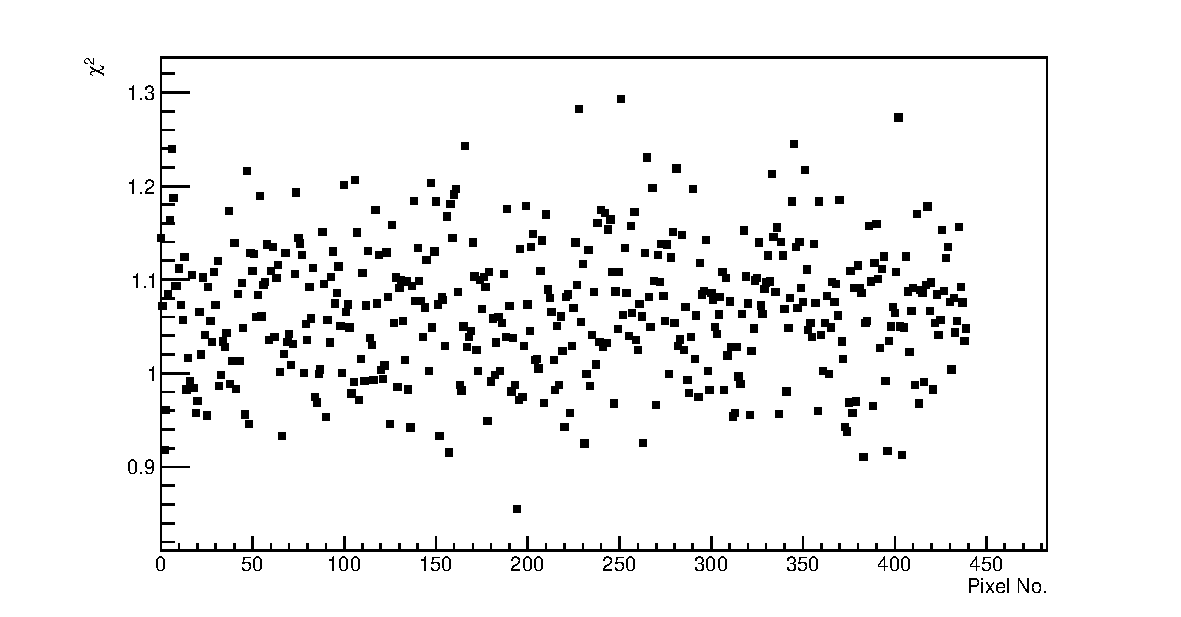
\includegraphics[width=\textwidth]{chapters/graphs/GainVarsMeas/LL_m04_2016-06-11/Set0and2/Chi2_AverageMethod_Signal_LowHV.pdf}
\caption{}
\end{figure}

\begin{figure}% Noise Chi2
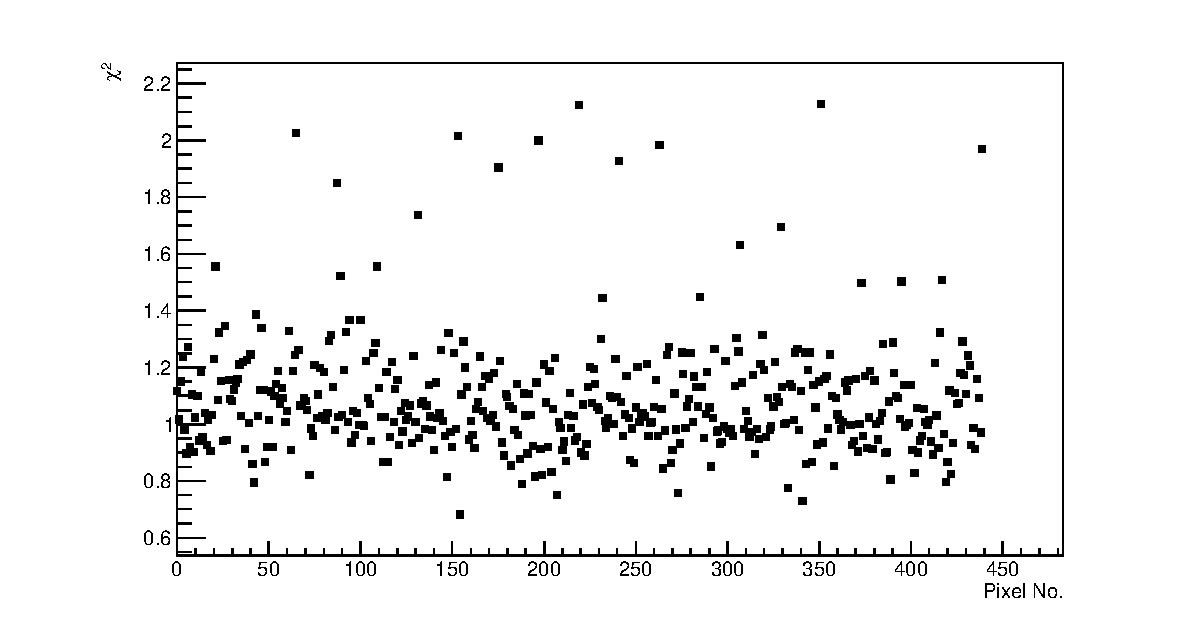
\includegraphics[width=\textwidth]{chapters/graphs/GainVarsMeas/LL_m04_2016-06-11/Set0and2/Chi2_AverageMethod_Noise_StandHV.pdf}
\caption{}
\vspace{3mm}
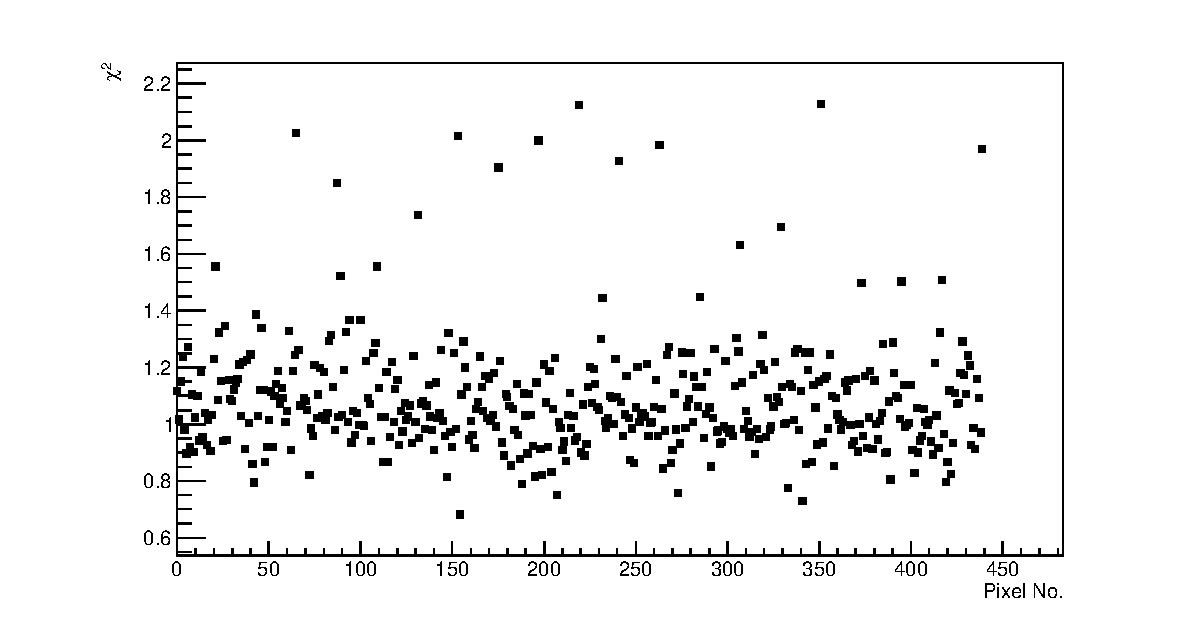
\includegraphics[width=\textwidth]{chapters/graphs/GainVarsMeas/LL_m04_2016-06-11/Set0and2/Chi2_AverageMethod_Noise_LowHV.pdf}
\caption{}
\end{figure}


\begin{figure} % Gain Variance Plot
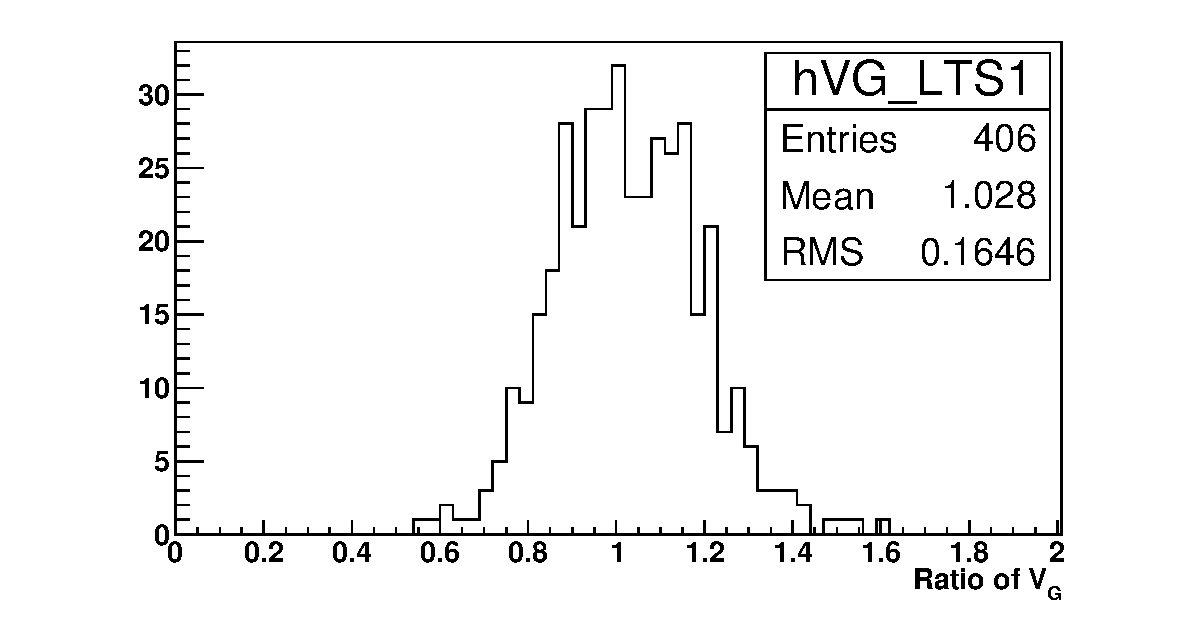
\includegraphics[width=\textwidth]{chapters/graphs/GainVarsMeas/LL_m04_2016-06-11/Set0and2/GainVairanceHist_Average_LTS.pdf}
\caption{}
\vspace{3mm}
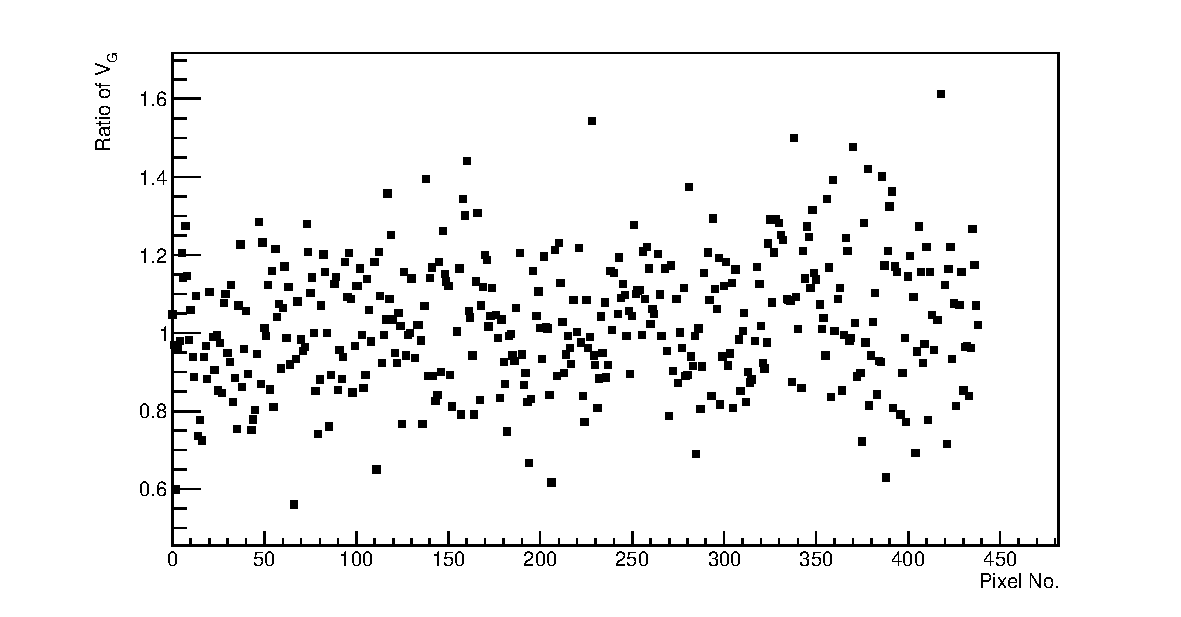
\includegraphics[width=\textwidth]{chapters/graphs/GainVarsMeas/LL_m04_2016-06-11/Set0and2/GainVars_Vs_Pixel_GainVariance_AverageLTS_Set0and2.pdf}
\caption{}
\end{figure}

\section{Result of Averaging Sets of Traces Method using Noise Distribution}

\begin{figure} % Gain Variance Plot
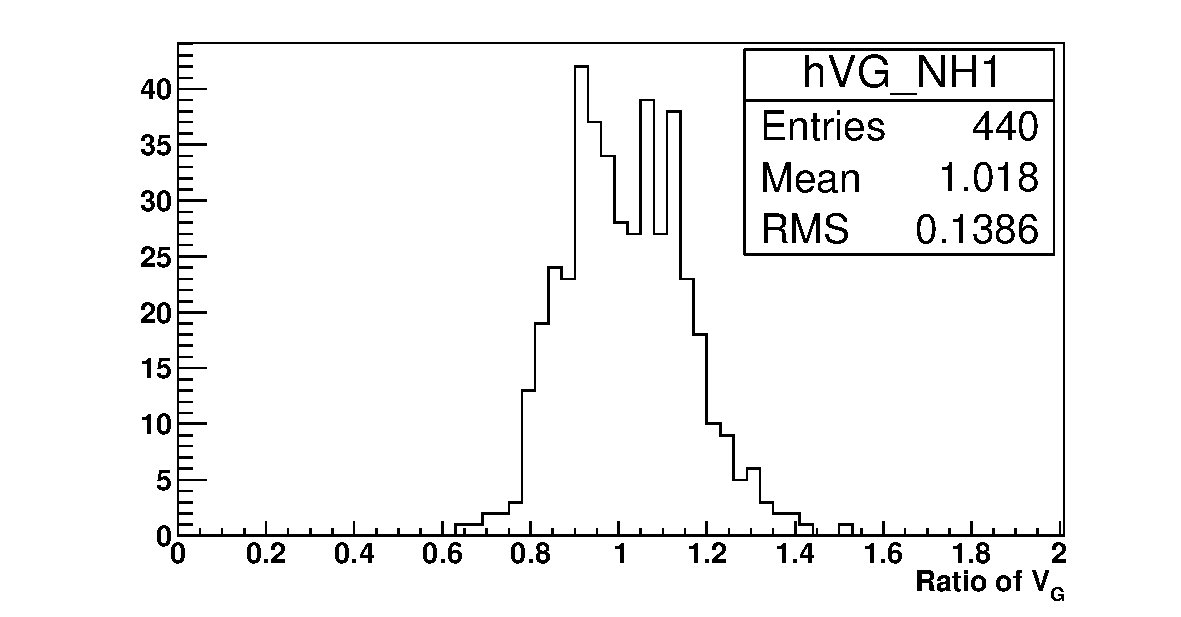
\includegraphics[width=\textwidth]{chapters/graphs/GainVarsMeas/LL_m04_2016-06-11/Set0and2/GainVairanceHist_Average_Method2.pdf}
\caption{}
\vspace{3mm}
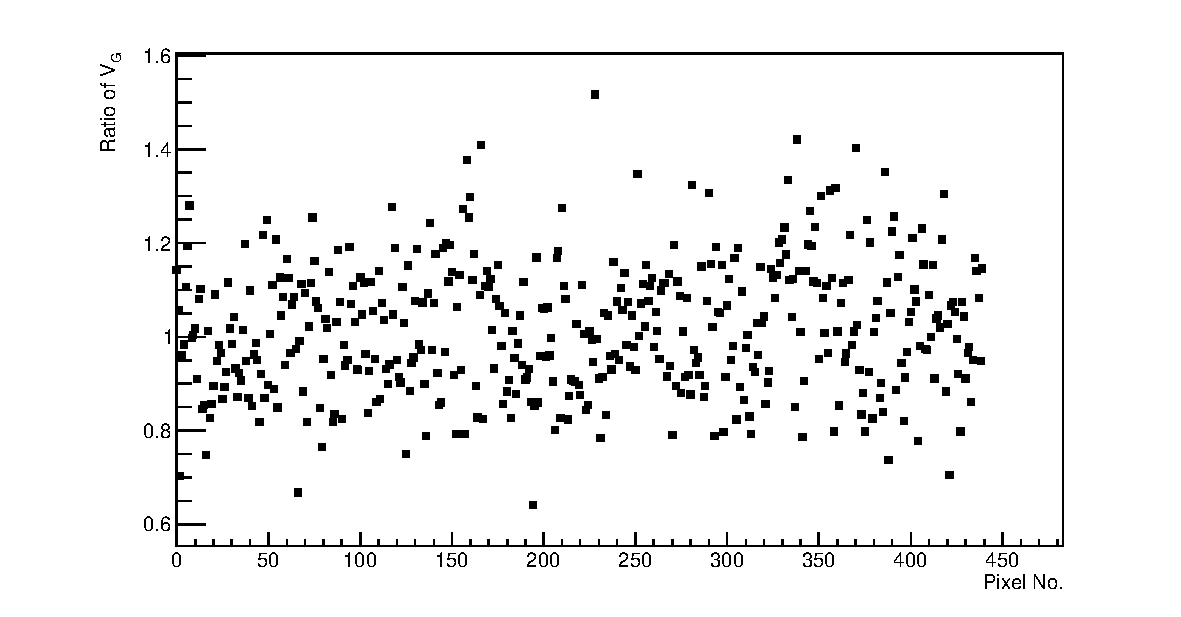
\includegraphics[width=\textwidth]{chapters/graphs/GainVarsMeas/LL_m04_2016-06-11/Set0and2/GainVars_Vs_Pixel_GainVariance_Average_Method2_Set0and2.pdf}
\caption{}
\end{figure}